\documentclass[a4paper]{report}
\usepackage[utf8]{inputenc}
\usepackage[numbers]{natbib}
\usepackage{hyperref}
\usepackage{graphicx}
\usepackage{datetime}
\usepackage{color}
\usepackage{microtype}
%\usepackage{draftwatermark}

%% Nicely format and linebreak URLs in the bibliography
\usepackage{url}

%% Nicer formatting of figure captions.
\usepackage[font=small,format=plain,labelfont=bf,up,textfont=it,up]{caption}

%\SetWatermarkScale{5}

%% Define a new 'leo' style for the package that will use a smaller font.
\makeatletter
\def\url@leostyle{%
  \@ifundefined{selectfont}{\def\UrlFont{\sf}}{\def\UrlFont{\small\ttfamily}}}
\makeatother
%% Now actually use the newly defined style.
\urlstyle{leo}

%\newcommand{\hi}[1]{{\color{red}\tiny \em #1\/}\\}
\newcommand{\todo}[1]{\footnote{{\color{red} {\bf TODO:} #1}}}

% ------------------------------------------------------------------------------
% Metadata
% ------------------------------------------------------------------------------
\title{Ontology Learning from Swedish Text}

\author{Jan Daniel Bothma}

\begin{document}

\maketitle

\abstract{
Ontology learning is the process of analyzing text to construct an ontology which represents the meaning encoded in the text.
Many methods have been proposed and evaluated for extracting concepts, relations, hierarchies and axioms from text, particularly for the earlier stages of the process.
Open questions in this field include researching new methods; exploiting social, structured and collaboratively curated data; evaluating, comparing and combining methods; scaling to larger corpora; supporting various and cross-language corpora; supporting ongoing ontology development; and improving user interaction.
This thesis contributes a survey of high level requirements for application and ongoing research of ontology learning, and applies several existing methods to learn ontologies from Swedish text.
This application is evaluated using \todo{which evaluation methods?}
}

\tableofcontents

\chapter{Introduction}

In this chapter we will introduce the concept of \emph{ontology learning} (OL), briefly identify some recent and significant work in OL and summarize open research questions identified in our literature review.
We will then propose the objective of this thesis along with research questions, how we intend to answer those questions, and delimitations to clarify the scope of this thesis. Finally, we will describe the layout of the remainder of this thesis report.

\section{Background}

A commonly-cited definition of ontologies in the field of knowledge engineering is as \emph{``a formal, explicit specification of a shared conceptualization''} \cite{StuderEtAl1998KEPM}.
Here, a \emph{conceptualization} is the objects, concepts and relations between them, in an abstract view of the world intended for a particular purpose.
The conceptualization should be \emph{shared} within the context of its application.
The objective with this explicit specification is to allow computer agents to operate on this view of the world or for its integration in human-operated software.
This is the sense of ontologies that this thesis is concerned with.
Ontologies have, for example, been applied in decision support systems, information bookmarking and retrieval, and in natural language processing.

Creating ontologies is a time-consuming and challenging process.
\todo{knowledge acquisition bottleneck}

The automatic or semi-automatic construction of ontologies is called Ontology Learning \cite{Cimiano06}.
Ontology Learning commonly involves some combination of preprocesing, term extraction, concept formation, concept hierarchy induction, non-taxonomic relation learning, and axiom extraction.
Most approaches to these tasks can be divided into being of logic, statistic or linguistic nature, as shown in Fig.~\ref{fig:tasktechout}\cite{Wong11Survey}.
\begin{figure}
  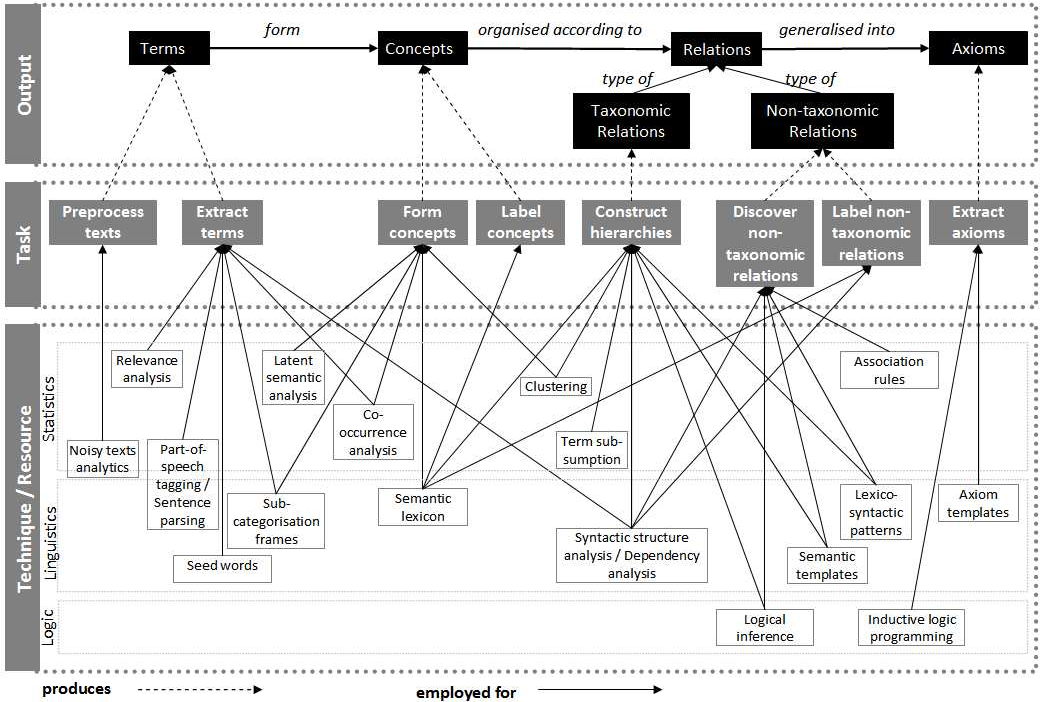
\includegraphics[width=\textwidth]{graphics/output-task-technique-WongLiuBennamoun.png}
  \caption{Tasks, techniques and outputs in ontology learning. Awaiting permission for reuse from \cite{Wong2009PhD}.}
  \label{fig:tasktechout}
\end{figure}
An additional task of ontology learning that is that of construction of the ontology from the extracted elements in a form suitable for its application.
This task is not necessarily strictly creating new ontologies, but is where ontology learning provides input of the greater ontology engineering process.
In this thesis we are avoiding the complexity of updating existing ontologies and other ontology engineering tasks, and \emph{simply} attempting to create new, valid\todo{perhaps define valid} ontologies.
\todo{Eva's explanation connecting with evaluation and OE is intuitively more realistic than Ciamiano's disconnected explanation}
\todo{give some examples of well-evaluated and newer techniques and their evaluation}

\section{Problem}

While many techniques for extracting terms and concepts have matured and have been evaluated against various competing techniques and in various settings, many areas of research are still somewhat unexplored.
Additionally, new technologies and on-line communities are providing new opportunities for supporting ontology learning.

Many existing methods rely on domain-specific models which need to be trained.
This training often involves manually annotated corpora which are time-consuming to produce, require domain expertise and aren't error-free.
There has been relatively little research in combining evidence from various languages.

\section{Objective}

given this background, the objectives of this thesis are

\begin{itemize}
  \item to provide a prototype system for learning domain ontologies from Swedish domain corpora
  \item to learn more about the tool framework needed to support application and ongoing research of Ontology Learning
\end{itemize}

\section{Research Questions}

We will fulfill these objectives by answering these research questions:

\begin{enumerate}
  \item{What are the general requirements for ontology learning research and application?}
  \item{How do common ontology learning methods need to be modified to extract ontologies from Swedish text?}
  \item{How do these modified methods perform compared to \todo{some baseline??? evaluation}?}
\end{enumerate}

\section{Approach}

To address these questions, we will...

\begin{itemize}
  \item produce a list of requirements
  \item sketch an architecture
  \item implement a prototype system
    \begin{itemize}
      \item reusing as much as possible
      \item describing how techniques had to be modified to work for Swedish
    \end{itemize}
  \item evaluate somehow
\end{itemize}

\section{Delimitations}

Ontological Architecture is how an ontology is constructed to be most useful where it is applied \cite{OntArchChapter}. While flexibility to support architectural decisions was considered, this area was not thoroughly researched in this thesis.

The prototype is intended to elicit issues where the proposed requirements and architecture can be improved upon.
It is not intended to be the final platform implementation.

The implications of following one school of thought in meaning representation with regard to semantic parsing (e.g. Davidsonian \cite{DavidsonianSemantics}) over another have not been taken into account.
This factor is expected to introduce some bias in the knowledge extracted, but the lack of thorough investigation of its implications on the requirements discussed in this research is a limitation of this work.

\section{Report Structure}

The rest of this report will be structured as follows:

\chapter{Ontology Learning}

This chapter reviews the state of Ontology Learning research.
We will discuss several end-to-end ontology learning systems which propose novel approaches to the problem, several approaches to particular ontology learning tasks.
Finally, shortcomings and suggested research areas identified in existing research will be summarized.

An interesting new approach is described in \cite{Poon2010OntoUSP}...
\begin{itemize}
  \item{input is dependency parse}
  \item{output is formulas representing classes, relations, clusters of those}
  \item{evaluation was based prepossessing with domain-trained syntactic parser}
\end{itemize}

\chapter{Application to Swedish Text}

\section{Architecture and High Level Design}

In this chapter we will discuss the design and implementation of a prototype system for automatically or semi-automatically extracting a domain ontology from domain-specific corpora in the Swedish language.

\section{Preprocessing Swedish text}

\section{Term Extraction}

\section{Concept Formation}

\section{Concept Hierarchy}

\section{Relation Extraction}

\section{Ontology Construction}

Here we describe how the evidence from the various stages can be use to build an ontology ready for validation.

\section{Method evaluation}

\chapter{Evaluation Method}


\chapter{Evaluation Results}


\chapter{Conclusion}


\chapter{Further Work}


\nocite{*}


\clearpage
%\addcontentsline{toc}{chapter}{References}
%\renewcommand\bibname{References}

%\renewcommand{\refname}{}
%\chapter{References}
\bibliographystyle{unsrtnat}
\bibliography{report}

\end{document}
